\documentclass[11pt]{article}

% NAACL 2027 Industry Track submission (review mode: anonymous, line numbers,
% page numbers). The arXiv version lives in ../main.tex and is unchanged.
% Tables in tables/ are generated by make_tables.py; do not hand-edit them.
\usepackage[review]{acl}

% Work around a lineno v5.6/v5.7 (2026-02) regression on LaTeX formats from
% 2025-06-01: its build/column/before hook writes each column tag to the .aux
% one column late, so every right-hand column is numbered as a left one and
% its numbers land in the gutter. The stock ACL template shows the same fault
% on TeX Live 2026. The tag the hook writes is read for the lines AFTER it, so
% we write the column that follows instead. acl.sty itself is unmodified, and
% older lineno versions (Overleaf, TeX Live <= 2025) never take this branch.
\makeatletter
\ifdefined\IfFormatAtLeastTF
\IfFormatAtLeastTF{2025-06-01}{%
  \@ifpackagelater{lineno}{2026/02/11}{%
    \RemoveFromHook{build/column/before}[lineno]%
    \AddToHook{build/column/before}{%
      \protected@write\@auxout{}{%
    \string\def\string\@LN@column{\if@firstcolumn2\else1\fi}}}%
  }{}%
}{}
\fi
\makeatother

\usepackage{times}
\usepackage{latexsym}
\usepackage[T1]{fontenc}
\usepackage[utf8]{inputenc}
\usepackage{microtype}
\usepackage{xurl}
\usepackage{inconsolata}
\usepackage{graphicx}
\usepackage{booktabs}
\usepackage{array}
\usepackage{tikz}
\usetikzlibrary{positioning,fit,backgrounds,shadows,arrows.meta}
\usepackage{listings}
\lstdefinestyle{promptstyle}{
  basicstyle=\scriptsize\ttfamily,
  breaklines=true,
  breakatwhitespace=false,
  breakindent=0pt,
  postbreak=\mbox{$\hookrightarrow$\space},
  columns=fullflexible,
  keepspaces=true,
  showstringspaces=false,
  frame=none,
  xleftmargin=0pt,
  aboveskip=4pt, belowskip=4pt,
  literate={—}{{---}}1 {–}{{--}}1 {≤}{{$\leq$}}1 {→}{{$\rightarrow$}}1
  {“}{{``}}1 {”}{{''}}1 {‘}{{`}}1 {’}{{'}}1 {…}{{\ldots}}1
  {≥}{{$\geq$}}1 {×}{{$\times$}}1 {½}{{$\frac{1}{2}$}}1
}

% Marks figures that come from deployment logs and engineering notes rather
% than from a recorded evaluation artifact (see the opening of Section 6).
\newcommand{\elog}{\textsuperscript{$\ddagger$}}

\title{Classify by Position, Not by Label: Deploying an LLM Pipeline\\
to Make US Early Learning Standards Machine-Readable}

\author{Anonymous submission}

\begin{document}
\maketitle

\begin{abstract}
  US states publish early learning standards for preschool children largely as PDFs, each formatted differently, so they are unavailable as structured data. We describe a deployed LLM pipeline that converts these documents into one schema. The hardest part is the hierarchy: a standard only makes sense under its domain, strand and sub-strand, and the clues to that structure (label words, code formats, number of levels) vary by state. One inexpensive model call infers each document's depth map (its nesting levels and how each looks on the page), then every element is classified by its position in that map, without state-specific code. On annotated excerpts from six states, recall is 1.000 at every level in the recorded run (at least 0.978 in repeats), and an audit of 297 detections finds one hallucination. Without the depth map, recall drops at the middle levels, which only position can identify, and a rule-based extractor matches ours only at the top level. Inference for a complete state document costs about \$4. Deployment taught us to compute database keys in code, not with the LLM, validate records before storage, test the batched production path, and check document coverage even when a run reports success.
\end{abstract}

% =====================================================================
\section{Introduction}
\label{sec:introduction}

Early learning standards are the developmental expectations that shape
curriculum, assessment, and teacher preparation for children before
kindergarten entry. More than fifty US jurisdictions issue these standards for
preschool-age children~\citep{ncecqa_elgs} and each jurisdiction designs its own document. Unlike K--12 academic standards, which have machine-readable exchange
formats~\citep{sutton2008achievement,1edtech2017case}, early learning standards
exist almost entirely as PDFs with multi-column tables, age-banded grids, and prose that are generally unique to each jurisdiction. Curriculum-planning tools, alignment
studies and cross-state comparisons all need standards as structured data, and
that data has been produced by hand~\citep{scottlittle2006conceptualization}, if at all.

Reading the text is the easy part. A standards document is a \emph{tree} rendered as a page, and an indicator means something only through its ancestry (its domain, strand, and sub-strand) and its age band. Recovering the tree means deciding how deeply every line is nested within the hierarchy. The surface cues that would help make that distinction vary widely between documents. Arizona writes \texttt{Strand 1: Language and Literacy}, Kentucky writes \texttt{Benchmark 1.1}, Nevada prints a code namespace that skips a level, and Colorado has no sub-strand tier at all. Rules tuned to one document's vocabulary tend to fail on the next and no
annotated corpus of parsed standards exists from which to learn the mapping.

We describe a system that recovers this structure with in-context LLM calls and is deployed as a serverless pipeline on AWS. The system's central idea is to recover structure from nesting position rather than from labels. A first, cheap pass infers a per-document depth map, then classifies every element against that map. \texttt{Benchmark 1.1} does not need to be recognized as a ``sub-strand'', only as sitting one level below \texttt{Language and Early Literacy Standard 1}. A parser resolves the detected elements into one canonical schema with deterministic identifiers, a validator guards the database, and a human can review every stored record in an editorial interface. The system runs end-to-end in production infrastructure and is in pre-launch use as the data layer behind a standards explorer.

\paragraph{Contributions.} (1)~A two-pass detection method based on
per-document depth-map inference, with no per-state code path, and a parser
that resolves six independently designed documents into one schema with
reproducible primary keys (\S\ref{sec:method}). (2)~An evaluation on six
states covering quality, an ablation, a rule-based baseline, run-to-run
stability, and whole-document scale and cost (\S\ref{sec:eval}). (3)~Lessons
from deployment centered on where a sampling model must not be trusted and
where failures hide (\S\ref{sec:lessons}).

% =====================================================================
\section{Related Work}
\label{sec:related}

\paragraph{Document hierarchy.} Between them, scholarly-PDF parsers,
layout-analysis toolkits, OCR-free transcribers, and open-source PDF
converters~\citep{lopez2009grobid,shen2021layoutparser,blecher2024nougat,auer2024docling,wang2024mineru}
recover text, page objects, and generic section headings, but not which
heading is a domain, strand, or sub-strand, or which printed codes identify a
standard. Hierarchical document parsers learn logical trees from large annotated
corpora~\citep{ma2023hrdoc,wang2024detect,xing2024dochienet}, but no such
corpus exists for standards documents, and their layouts vary by state.
Closest to ours, HiPS~\citep{wehnert2025hips} segments books from
table-of-contents metadata or an LLM-refined pipeline, and DocsRay~\citep{jeong2025docsray} prompts an LLM for a pseudo
table of contents.
Our depth map lists no headings: it describes how many levels a document uses
and how each looks, is inferred zero-shot, and is the authority for every
classification.

\paragraph{LLMs for extraction and in production.} LLM extraction is
competitive with supervised methods when labels are
scarce~\citep{agrawal2022large,xu2024large}. GoLLIE~\citep{sainz2024gollie}
trains models to follow annotation guidelines, whereas we give a frozen model
document-agnostic structural rules in the prompt. We validate and repair JSON
instead of constraining decoding~\citep{willard2023efficient,tam2024speak} and check
structural invariants before storage, as \citet{aggarwal2025fiscal} do with
the hierarchical totals of fiscal tables. Temperature zero does not make LLM
output repeatable~\citep{ouyang2025nondeterminism,atil2025nondeterminism}, and
our lessons (\S\ref{sec:lessons}) add to practitioner accounts of production
ML~\citep{shankar2024operationalize} and to work on LLM-pipeline
assertions~\citep{shankar2024spade}.

\paragraph{Machine-readable standards.} ASN~\citep{sutton2008achievement} and
CASE~\citep{1edtech2017case} provide a data model and an exchange format for
K--12 standards. Work aligning instruction, tests and resources to standards
takes them as given, already structured or coded by
hand~\citep{porter2002measuring,polikoff2011howwell,devaul2011computer,xu2025automated}.
We know of no normalized early-childhood set, and the one federal framework
only applies to Head Start~\citep{ohs2015elof}.

% =====================================================================
\section{Schema and Data}
\label{sec:data}\label{sec:corpus}\label{sec:schema}

\paragraph{Canonical schema.} The target schema has four levels,
\emph{domain}, \emph{strand}, \emph{sub-strand} and \emph{indicator}, of which
the middle two are optional because not every document uses all four. Colorado publishes no sub-strand tier, and forcing one would mean inventing structure. Each level has a code, a name and an optional description.
The indicator also carries an age band, a source page, and the verbatim source
text. The unit of storage is a leaf with its full lineage, identified by
\texttt{\{country\}-\{state\}-\{year\}-\{indicator\_code\}}, where the indicator
code is fully qualified and carries any side-by-side disambiguator itself:
an age column appends its month range (Texas \texttt{I.A.2.36-48} vs.\
\texttt{I.A.2.48-60}, and likewise California's age columns), and a
proficiency column its label (California \texttt{ELD.1.0.VOCA.1.1.DISC}). Because the identifier is a primary key, it must be reproducible from the document alone, regardless of the order the pipeline processed it in. Every level also carries a human-verification state
(Appendix~\ref{sec:appendix-schema}).

\paragraph{Corpus and tiers.} We use documents from six states: four for development (AZ, CA, CO, TX) and two for validation (NV, KY). No code path names any state, but validation-state failures prompted several general fixes during development, so the set is \emph{not} a clean held-out test (see Limitations). Each document exists at up to three tiers. The \emph{full} tier is the published PDF. The \emph{trimmed} tier removes front matter, essays, and appendices but \textbf{retains every standard}. This reduces cost but not coverage. The \emph{subset} tier is one to two domains per state, 70 pages and 262 standards in total, annotated for grading (\S\ref{sec:eval}). \textbf{All headline quality numbers are at this tier.} Both the subset and trimmed tier cuts were made by hand. Appendix~\ref{sec:appendix-corpus} lists every source document and the retained pages.

% =====================================================================
\section{System}
\label{sec:method}

The pipeline has six stages. \emph{Ingestion} registers a PDF.
\emph{Extraction} recovers text blocks with page coordinates from Textract OCR
repaired against the PDF's own text layer. \emph{Detection} emits a flat list of
typed elements. \emph{Parsing} resolves them into the schema.
\emph{Validation} checks structural invariants. \emph{Persistence} writes
surviving records to PostgreSQL. The stages are Lambda functions that exchange JSON
through S3, so any stage can be replayed in isolation. Detection and parsing
are batched through a prepare~$\rightarrow$~Step Functions
\texttt{Map}~$\rightarrow$~merge pattern (at most three concurrent workers) so
that a long document does not exhaust a function timeout
(Appendix~\ref{sec:appendix-architecture}).

\paragraph{Detection and parsing.} Detection decides \emph{what is on the page}, a local judgment, and parsing decides \emph{what each element is a child of}, a global judgment, since a parent may be printed pages earlier within the document. Each stage sees the context it needs (parsing reasons over a whole domain at once), is graded against its own gold annotations (its \emph{golden}), and runs on the cheapest adequate model: the depth-map pass on Claude Haiku~4.5, detection on Claude Opus~4.6, parsing on Claude Sonnet~4.6, all at temperature zero.

\subsection{Detection}
\label{sec:method-detection}

\paragraph{Pass 1: depth map.} One call infers how many nesting levels the document uses and how each one looks on the page (Appendix~\ref{sec:prompt-depthmap}). Detection later assigns every element's level from this map, so \emph{a level missing from Pass~1's input is missing from the whole run}. Pass~1 sees a 6{,}000-token sample of the extracted text blocks, and how that sample is drawn is relevant. Headings are rare and prose is abundant, so taking every $n$th block drops the lines that establish the top of the hierarchy (\S\ref{sec:lessons}). Because indentation tracks nesting, a rare horizontal position usually marks a rare level. We therefore group blocks by their left edge and give each group at least twelve blocks spread across the document, filling the rarest groups first. The rest of the budget samples the remaining text, also spread evenly.

\paragraph{Pass 2: classification.} The document is chunked into ${\sim}$2{,}000
token windows with 500 tokens of overlap, and each chunk is classified with the
depth map as context. The central instruction is to classify each element by where it sits in the map rather than by its label word
(Appendix~\ref{rule:positional}). Supporting rules are equally general. In a \texttt{<Label> <id>: <Title>} heading, the label and id form the code for \emph{any} label word, and a printed code is authoritative whether it appears inline, in a
caption, or as the shared prefix of the element's descendants' codes. If the document does not print a code, one is derived from the title by a fixed
abbreviation procedure (Appendix~\ref{rule:code-resolution}).

\subsection{Parsing and identifiers}
\label{sec:method-parsing}

% Table 1 belongs to Section 5, but a full-width float can appear at the
% earliest on the page after the one that defines it, so it is input here to
% land at the top of the page where Section 5 begins.
% AUTO-GENERATED by paper/naacl2027/make_tables.py -- do not hand-edit.
% Source: paper/results/task1_20260826/summary.json, task2_20260826/summary.json, the signed FP audits, corpus_tiers.json
% Regenerate with: python paper/naacl2027/make_tables.py
\begin{table*}[t]
  \centering
  \small
  \begin{tabular}{lrrrrrrr}
    \toprule
    & & & \multicolumn{2}{c}{\textbf{Detection}} & \multicolumn{3}{c}{\textbf{Parsing}} \\
    \cmidrule(lr){4-5} \cmidrule(lr){6-8}
    \textbf{State} & \textbf{pp} & \textbf{Std.} & \textbf{Ver.\ prec.} & \textbf{Code acc.} & \textbf{Coverage} & \textbf{Field acc.} & \textbf{Fully corr.} \\
    \midrule
    AZ & 15 & 45 & 1.000 & 4/4 & 18/18 & 0.997 & 17/18 \\
    CA & 13 & 94 & 1.000 & 25/25 & 21/21 & 1.000 & 21/21 \\
    CO & 10 & 48 & 1.000 & 7/7 & 9/9 & 1.000 & 9/9 \\
    TX & 9 & 25 & 1.000 & 8/8 & 8/8 & 1.000 & 8/8 \\
    \midrule
    NV & 15 & 24 & 0.981 & 46/46 & 24/24 & 1.000 & 24/24 \\
    KY & 8 & 26 & 1.000 & 44/44 & 26/26 & 1.000 & 26/26 \\
    \bottomrule
  \end{tabular}
  \caption{Quality per state at the \emph{subset} tier (\S\ref{sec:data}), from one recorded run. NV and KY, below the line, are the validation states. \emph{pp}: subset pages. \emph{Std.}: standards the parser produced. \emph{Ver.\ prec.}: verified precision (\S\ref{sec:eval}). The fractions count golden items. \emph{Code acc.} is matched golden elements whose code is correct, \emph{Coverage} is golden standards the parser produced, and \emph{Fully corr.} is golden standards with every field correct. \emph{Field acc.} is the share of graded fields that match. Development-state goldens are spot checks, so their counts are small. Detector recall (1.000) and the Pass-1 level count (matching the golden) were the same in every state and are not shown. NV results vary across repeat runs (\S\ref{sec:eval-stability}).}
  \label{tab:headline}
\end{table*}


Parsing composes each indicator's qualified code from its ancestors, and printed namespaces are not uniform. Nevada's sub-strand code does not extend its strand's, so requiring it would corrupt all 24 Nevada standards. Kentucky's \texttt{Benchmark 1.1} restates its parent inside its own id, so naive composition counts the parent twice. Each case is handled by a rule that reads code \emph{shape} rather than vocabulary. The parser peels an ancestor's code off a descendant's until the namespace stops, keeps a level's own id when its peeled code matches the level below, never re-qualifies an already-qualified code, collapses a dotted child that repeats its parent's last segment, and declines any repair that cannot be verified against the row's own ancestry or would introduce whitespace (Appendix~\ref{sec:prompt-parsing}).

Uniqueness is enforced after the batch merge because collisions can span batches. Rows that share a code each gain segments from their own ancestors' codes and rewriting all of them makes the result order-independent. A numeric suffix in document order is a logged last resort. Finally, the validator rejects any record whose codes contain whitespace, whose indicator code does not extend its nearest ancestor's, or whose identifier does not end in that code.

\subsection{Dividing work between prompts and code}
\label{sec:method-llm-first}

An earlier revision scored strongly on the development states by accumulating per-state logic: regular expressions for label words, a collision special case, and an abbreviation helper tuned to one state. However, it transferred poorly to new documents. We removed that logic and adopted a rule: structural decisions stay in the prompt, stated as general principles about documents, and Python may read only the \emph{shape} of an output (dot segments, whitespace, containment, layout position), never a document's words. We treat any new per-state branch as a regression, even when it raises a score.

We keep deterministic code only when a prompt rule cannot reach zero error; the code then executes the same rule the prompt states rather than a competing one, so the prompt lowers the error rate and the code removes what remains (\S\ref{sec:lessons}, lesson~1). Fifteen of the prompts' worked examples are, however, distinctive to one state's golden, including four Kentucky strings and one Nevada string illustrating the abbreviation procedure.

% =====================================================================
\section{Evaluation}
\label{sec:eval}

\paragraph{Protocol.} Two suites grade the stages separately: the detector against flat-element goldens and the parser against nested normalized-standard goldens. Development-state detector goldens are spot checks (5--25 elements), so an unmatched detection is usually an annotation gap rather than an error. Raw precision on those states mostly measures annotation coverage. We therefore report \emph{verified precision}, which counts a detection as an error only if its element is absent from the source. We checked by hand every in-scope detection the golden does not match, 162 of 297. Kentucky's golden is exhaustive, so its precision is a true hallucination rate. The suites exercise the direct, unbatched path. The batched production path is evaluated separately at scale (\S\ref{sec:eval-scale}). A script regenerates every tabulated number from a recorded run artifact.

\subsection{Quality on six states}
\label{sec:eval-headline}

Table~\ref{tab:headline} displays the results. In the recorded run, detector recall is 1.000 at every level in all six states, including both validation states. The 135 pooled golden elements give a 95\% lower bound of 0.973 (Clopper--Pearson), and Nevada's recall falls to 45/46 in some repeats (\S\ref{sec:eval-stability}). In every state, Pass~1 infers the same number of levels as the golden. The audit finds one hallucinated element (verified precision 0.997 pooled): a Nevada indicator emitted a second time from a truncated transcription of a multi-column table, with an invented clause appended. The parser covers every annotated standard and its uniqueness resolver, which logs when it acts, never had to separate two standards in the 29 subset-tier runs whose logs were retained.

\subsection{Ablation and baselines}
\label{sec:eval-ablation}

% AUTO-GENERATED by paper/naacl2027/make_tables.py -- do not hand-edit.
% Source: paper/results/task3_20260826/ablation_comparison.json, task4_20260826/baseline_comparison.json
% Regenerate with: python paper/naacl2027/make_tables.py
\begin{table}[t]
  \centering
  \small
  \begin{tabular}{lrrrr}
    \toprule
    \textbf{Level} & $n$ & \textbf{Full} & \textbf{No map} & \textbf{Rule-based} \\
    \midrule
    domain & 13 & 1.000 & 1.000 & 1.000 \\
    strand & 25 & 1.000 & 0.920 & 0.240 \\
    sub-strand & 24 & 1.000 & 0.833 & 0.667 \\
    indicator & 73 & 1.000 & 1.000 & 0.137 \\
    \bottomrule
  \end{tabular}
  \caption{Detector recall by hierarchy level, pooled over six states: the full method, the method with the Pass-1 depth map ablated, and a rule-based extractor graded by the same suite. Subset tier; ablation off-arm recall varies by run (\S\ref{sec:eval-ablation}).}
  \label{tab:levels}
\end{table}


\paragraph{Depth map.} Disabling Pass~1 makes the detector revert to the no-map path it already uses when inference fails. Without the map, domain and indicator recall stay at 1.000, while strand recall falls to 0.920 and sub-strand recall to 0.833 (Table~\ref{tab:levels}). The surviving levels have distinctive surface forms (a document's top division and its numbered leaves). The levels that degrade are those identifiable only by what they sit between in the document.

On Kentucky, the map-on arm reproduces the golden's 3/5/10/26 elements per level exactly, while the map-off arm emits 4/10/6/26 because it promotes \texttt{Benchmark N.N} items to strand on the strength of their label. The direction is fixed across three runs per arm per state, but the magnitude is a draw (Kentucky off-arm recall 0.89--0.98, Colorado 0.71--0.86). Texas keeps recall and loses code accuracy instead (8/8~$\rightarrow$~5/8).

\paragraph{Rule-based extractor.} A deterministic extractor was built on numbering
patterns, capitalization, indentation, and line shape. The extractor was developed against the
four development states, and graded by the same suite, ties the LLM at domain
(13/13), and collapses below it (Table~\ref{tab:levels}). Almost all of its errors are omissions rather than mislabelings. On Kentucky, it never emits 31 of 44 golden elements, but it misplaces none. Even on the development states, its recall is 0.57--0.80.

\paragraph{One whole-document prompt.} One call per document, with the same prompt, model, and grader but no depth map, chunking, or repairs, matches the method on Arizona and Nevada. It loses code accuracy on Kentucky (44/44~$\rightarrow$~28/44) and Texas (8/8~$\rightarrow$~5/8), each missing a different primary key for the same standard, and loses recall on Colorado (0.429). California fails entirely because its call stopped at exactly the 16{,}000-token output cap, which truncated the JSON so that nothing parsed. Arizona succeeded within 11\% of the same cap. Chunking limits this loss to one chunk, which makes it necessary at full-document scale. This arm is one draw per state.

\subsection{Stability}
\label{sec:eval-stability}

We re-ran both suites five times per state on frozen inputs with caching disabled, split across two days. Matched by title, 5 of 304 detected elements and 9 of 201 parsed indicators differ between runs, all in four places. Four detector differences are elements outside the goldens that some runs omit (three Arizona sub-strands, one Nevada indicator) and the fifth is Nevada's domain code, which alternates between \texttt{S} and \texttt{Science}. Nevada's parser places 4 indicators under a sibling strand (e.g., \texttt{SS.1} for \texttt{SS.2}), each in one run, and gives a fifth a sibling sub-strand's name. California's parser intermittently leaves a structural label inside an indicator code (\texttt{ELD.1.0.VOCA.Foundation 1.1.BROA}), on 12 rows across 4 indicators. All 12 malformed codes contain whitespace, and the validator rejected every one before persistence. The Nevada strand codes, by contrast, are well formed, so no shape check can catch them.
Splitting the runs across days mattered. Nevada's detector was identical in three runs
one evening and dropped that indicator in both runs the next day. In
five further runs it missed one golden indicator twice (recall 45/46). Nevada's recorded detector
code accuracy of 46/46 did not reproduce: five runs give 44--45.

\subsection{Scale and cost}
\label{sec:eval-scale}

% AUTO-GENERATED by paper/naacl2027/make_tables.py -- do not hand-edit.
% Source: paper/results/task6_20260830/manifest.json
% Regenerate with: python paper/naacl2027/make_tables.py
% Corpus tier: _trimmed -- every standard in the document, non-standards matter removed. NOT the full published PDF and NOT the _only_subset tier.
\begin{table}[t]
  \centering
  \small
  \setlength{\tabcolsep}{4pt}
  \begin{tabular}{lrr}
    \toprule
    & \textbf{KY} & \textbf{CO} \\
    \midrule
    Pages & 52 & 41 \\
    Detection chunks / batches & 18 / 4 & 17 / 4 \\
    Parse batches & 9 & 9 \\
    Elements raw $\rightarrow$ merged & 363$\rightarrow$329 & 390$\rightarrow$300 \\
    LLM calls & 45 & 45 \\
    Input / output tokens (k) & 379 / 150 & 390 / 131 \\
    Wall clock & 13m19s & 9m52s \\
    \midrule
    \textbf{Inference cost (USD)} & \textbf{\$4.41} & \textbf{\$4.02} \\
    \quad depth map (Haiku 4.5) & 0.3\% & 0.5\% \\
    \quad detection (Opus 4.6) & 59\% & 57\% \\
    \quad parsing (Sonnet 4.6) & 40\% & 42\% \\
    \bottomrule
  \end{tabular}
  \caption{One batched production run per document at the \emph{trimmed} tier, which keeps every standard (\S\ref{sec:data}). Cost is model inference only, at Bedrock on-demand rates confirmed in August--September 2026, excluding Textract OCR and fixed infrastructure.}
  \label{tab:scale}
\end{table}


The subset tier never exercises batching, since every document fits in one batch. Table~\ref{tab:scale} reports one production run each on Kentucky's and Colorado's complete standards (trimmed tier): 17--18 detection chunks in four batches, merges that remove 34 and 90 duplicate elements, about \$4 of model inference (Textract OCR adds \$0.6--0.8), and 10--13 minutes per document, with no throttling or rejected records. Detection is the main cost (57--59\%), while the depth-map pass costs 0.3--0.5\% of a run.

To grade quality at this scale, we annotated Kentucky's complete trimmed tier (277 elements, 207 standards). We started from one run's output, checked every element against the published PDF, and searched the PDF for elements no run emitted. On a document with $6.5\times$ the subset's page count, three further runs each find all \textbf{277 of 277} elements and emit no ungrounded element. Scale does introduce one defect the subset never shows. Kentucky prints a \texttt{THREE AND FOUR YEAR OLDS} page banner, which the detector attaches to 164 elements as their own age band in each of three runs (159 of them the same elements). Deduplication keys on age band, so ${\sim}$15\% of detector output survives as banded/unbanded duplicates, which collide in parsing and receive numeric-suffix identifiers: 10--11 fabricated primary keys per run, and naming standards that do not exist. Parser field accuracy holds at $0.995\pm0.002$, but coverage ranges from 0.81 to 0.93. Colorado, which has no banner, shows zero duplicates and zero fabricated keys over 240 standards.

% =====================================================================
\section{Lessons from Deployment}
\label{sec:lessons}\label{sec:method-confidence}\label{sec:experiments-confidence}

Figures marked \elog\ come from production logs and engineering notes kept
during development, not from the recorded evaluation artifacts behind
\S\ref{sec:eval}.

\paragraph{1. Do not let the model execute an algorithm that feeds a key.} The title-abbreviation procedure (\S\ref{sec:method-detection}) is a deterministic string algorithm, yet a temperature-zero model samples it. Across three detector runs on one frozen Kentucky extraction, 11 of 44 elements received a different code at least once\elog, while level, page, and age band never varied. Across three parser runs, 58\% of Kentucky's \texttt{standard\_id}s, which are database keys, changed\elog. We now run the procedure in Python, but only where the document printed no code, using two shape checks: the code is all uppercase letters and it does not appear in the element's own source text. It reproduces all 40 hand-annotated derived codes. More generally, we let the model make judgments and move anything with a single correct output into code.

\paragraph{2. Enforce correctness where data is persisted.}
Composed codes are right most of the time, which is not good enough for a key,
so the validator rejects structurally impossible records. It had zero false positives on all 262 subset
standards and blocked every historical defect row\elog.
Its rules are deliberately narrow. Requiring every level, not only the leaf, to extend its parent would reject all of Nevada. Rejections can also expose an upstream error. When Pass~1 lost a level on Kentucky's complete document, the validator correctly rejected 102 of 202 standards\elog\ because their codes had nothing to be qualified against, although the fault was two stages upstream.

\paragraph{3. A successful status can hide a failed run.} A temperature-zero model intermittently returns \texttt{"code": null} for a required field, and retries cannot help because they resend the identical prompt. On one Kentucky production run, one such element per chunk raised a schema error inside the per-element loop, discarding every valid element in its chunk, and the worker's three retries failed identically. The execution reported \texttt{SUCCEEDED}, with no Step Functions retries and no throttling, while 12 of 18 detection chunks were lost, and records were persisted from only 40\% of the document\elog. The fixes were small (deriving the missing code in Python and isolating per-element failures), but stage status still does not propagate into execution status. We now check element and page coverage by hand after every run. Automating that check is open work.

\paragraph{4. Evaluation and production took different code paths.} Evaluation
runs detection and parsing directly. Production batches them and merges the
results. The resolver that keeps primary keys distinct ran on the direct path but not in the batched merge, so a Kentucky production run stored two distinct indicators
under the same key\elog. Conversely, rejoining a description split
across overlapping chunks does nothing in evaluation, where the description
falls in one chunk. In production, however, it restored a 3{,}500-character Nevada
description\elog. The merge now runs the direct path's final steps too.

\paragraph{5. Small inputs hide structural failures.} The every-$n$th Pass~1
sampler worked on every subset document because each fell under the token
budget and was never sampled. On Kentucky's complete document it kept 2 of 9
section headings, Pass~1 reported three levels for a four-level document, and
zero sub-strands were emitted among 267 elements\elog. With layout-stratified
sampling, Pass~1 keeps 9 of 9 and reports four levels stably across three runs\elog.

% =====================================================================
\section{Conclusion}
\label{sec:conclusion}

Classifying elements by nesting position rather than by label recovers the hierarchy of six independently designed early learning standards documents with no per-state code, at about \$4 of model inference per document. This makes it practical to turn every state's PDF into structured records a person can review, data that has been previously produced by hand, if at all. The system is already the data layer behind a standards explorer in pre-launch use.
Deployment depended on never trusting a sampling model with anything that has one right answer (keys, invariants, run health) and on testing the system as it runs. We treated those checks as essential because our worst failures, a lost hierarchy level, most of a document discarded behind a \texttt{SUCCEEDED} status, and fabricated primary keys, never appeared on the evaluation subsets. The next test is a state seen only after development is frozen, and the goal is every jurisdiction.

% =====================================================================
\section*{Limitations}
\label{sec:limitations}\label{sec:discussion-limitations}

\paragraph{Tier.} Headline quality is measured on hand-trimmed subsets (70 pages);
whole-document quality is measured for one document (Kentucky) and no
document as large as Arizona's 217-page publication has been run end to end.

\paragraph{No held-out state.} Nevada and Kentucky were checked against during
development. Their failures motivated several general rules, and the prompts
carry five strings from their goldens, so their results are validation results rather than held-out ones.

\paragraph{Goldens.} Development-state detector goldens are spot checks, so only Kentucky provides a
precision figure that is a true hallucination rate. All goldens, and the hallucination audit are completed by a single annotator, so no inter-annotator agreement
is reported, and pooled recall rests on 135 golden elements.

\paragraph{Baselines.} All comparisons are internal: the depth-map ablation, a
rule-based extractor of our own, and a single-call prompt. No off-the-shelf
document parser was evaluated and the single-call arm is one run per state.

\paragraph{Nondeterminism.} The pipeline is not deterministic. Stability rates are lower bounds from five or
six runs, and one of our earlier recorded results did not reproduce.

\paragraph{Paths.} The quality suites grade the direct path and the batched path is graded only at scale.

\paragraph{Models.} All stages use one model family. No model-tier ablation or other provider was tested.

\paragraph{Extraction.} A heading that OCR fuses or drops cannot be recovered downstream. The one hallucination arose this way.

\paragraph{Known defect.} The age-band defect of
\S\ref{sec:eval-scale} is deliberately not repaired. Every recorded result is
keyed to a hash of the detector and parser source. The fix, a prompt rule
that a band comes from a column distinguishing siblings and never from a page
banner, would invalidate every measurement reported here. Deduplication should
also stop keying on a field this unstable.

\paragraph{Engineering-log figures} (\elog)
in \S\ref{sec:lessons} are not backed by archived evaluation artifacts.

\paragraph{Scope.} Six English-language US documents; we make no claim about other
document families or countries.

\section*{Ethical Considerations}
\label{sec:ethics}\label{sec:artifacts-statement}

\paragraph{Data.} The inputs are published policy documents from state
agencies. No student, teacher or family data and no human subjects are involved. The only people recorded are authenticated editors using the standards explorer, whose identity
comes from their session, never from a model.

\paragraph{Stewardship.} Standards shape curriculum and assessment so a
mis-extracted standard can propagate into materials that reach children. The
design therefore assumes a human will check every record and makes checking
cheap (source page on every record, per-level verification state). No record
skips review on the strength of the detector's confidence score
(Appendix~\ref{sec:appendix-confidence}) and the normalized records point back into the authoritative documents rather than replacing them. Using unverified output for anything with regulatory or
assessment weight would be a misuse. A queryable corpus also invites cross-state
comparisons the documents do not support: a state with fewer recorded
indicators does not have a lower bar for educational quality.

\paragraph{Artifacts.} State government works have no uniform public-domain
status, so we do not redistribute the source documents or the goldens derived from them. Appendix~\ref{sec:appendix-corpus} identifies each document so it can
be obtained from its agency. The complete text of all three prompts is
reproduced verbatim in Appendix~\ref{sec:appendix-prompts} and the schema and
annotated examples are in the other appendices. The implementation is not
released which limits reproduction to reimplementing the method from the
prompts and schema.

\paragraph{Use of AI assistants.} Following the ACL policy on AI writing
assistance, we disclose the following uses of Claude (Anthropic) as an
assistant. These are separate from the Claude models the pipeline itself calls
(\S\ref{sec:method}).

\emph{Code:} Claude Code was used as a coding assistant to implement the pipeline, evaluation harness, rule-based baseline, and scripts that generate all tables and appendices. The authors designed the system and experiments, reviewed the implementation, and are responsible for the correctness of the code, methods, and results.

\emph{Literature search:} Claude assisted the authors' literature search by suggesting candidate related work and drafting bibliography entries. The authors read each cited work, verified its relevance, and checked every bibliographic entry against its publisher or archive record.

\emph{Annotation support:} for the hallucination audit (\S\ref{sec:eval}), Claude generated provisional first-pass verdicts for unmatched detections based on the source PDFs. The drafting model belongs to the same family as the system under audit. The authors independently checked every proposed verdict against the source PDF and made all final annotation decisions; the authors are the annotators of record.

\emph{Writing:} The authors wrote the manuscript. Claude was used to edit it, revising text for clarity, concision, and consistency with the recorded results. The authors developed the research questions, system design, experiments, intellectual framing, and conclusions. They reviewed and verified all edited text, numerical claims, and citations and take responsibility for the final manuscript.

\bibliography{../references}

\appendix

\section{Prompts}
\label{sec:appendix-prompts}
% AUTO-GENERATED by paper/naacl2027/make_tables.py -- do not hand-edit.
% The listings are the complete text of paper/anc/prompts.txt, which
% paper/analysis/make_prompt_appendix.py renders from the live prompts.

This appendix and the schema of Appendix~\ref{sec:appendix-schema} are what this paper discloses in place of a code release (see Ethical Considerations). It reproduces the \textbf{complete text of all three prompts}, verbatim, exactly as the system emits them, with only the per-run document content replaced by a placeholder in angle brackets. The detection prompt is split into consecutive listings at the rules the body cites; nothing is omitted between them. Long lines are wrapped at the column edge (marked~$\hookrightarrow$).

\subsection{Pass 1: depth-map inference}
\label{sec:prompt-depthmap}
Run once per document, on a layout-stratified sample of text blocks (\S\ref{sec:method-detection}). Its output is supplied to every detection call as the authority for what each nesting level is.

\begin{lstlisting}[style=promptstyle]
You are analyzing the structural skeleton of an early learning standards document. You will NOT extract individual elements — only the document's nesting hierarchy.

Read the sample below and identify how many distinct nesting depths the document uses, what each depth looks like (its prefix/label pattern), and one concrete example. The DEEPEST depth is always the leaf (individual learning goals/foundations/benchmarks).

This document's depths must then be mapped to a canonical 4-level hierarchy:
- depth 1 → "domain"
- depth 2 → "strand"
- depth 3 → "sub_strand"
- deepest depth → "indicator"

Rules:
- Fill the canonical levels FROM THE TOP DOWN. The first depth is always "domain", the deepest depth is always "indicator", and any depth in between takes the next canonical level in order: the depth directly under domain is "strand", the one below that is "sub_strand". A document with fewer depths therefore drops the levels at the BOTTOM of that middle range — never "strand".
- A 4-level document (domain > group > sub-group > leaf) maps to: domain, strand, sub_strand, indicator.
- A 3-level document (domain > group > leaf) maps to: domain, strand, indicator. There is NO sub_strand — the single middle level is a STRAND, never a sub_strand.
- A 2-level document (domain > leaf) maps to: domain, indicator. There is no strand and no sub_strand.
- Use depth POSITION, not the document's labels. If a document uses "Sub-Strand" as the label for the second level (directly under domain), it is still a STRAND in our canonical hierarchy — and likewise a document that calls its single middle level "Section", "Concept", "Goal", or anything else still maps that level to "strand".

Every line is prefixed with its page and the horizontal position it was laid out at: `[Page N | x=0.09]`, where x is the line's left edge as a fraction of the page width. Use x to work out whether a page uses a side-by-side layout: lines of one column share nearly the same x, and a jump to a clearly different x means a different column. Lines you judge to be in the same column read as one continuous cell, even when lines from other columns are interleaved between them. Treat parallel columns as repetitions of ONE depth, not as separate depths.

Be deterministic and conservative. Do not speculate. If you cannot tell whether two depths are distinct, assume they are the same depth.

Output ONLY a JSON object with this exact shape:
{
  "doc_depths": [
    {"depth": 1, "canonical_level": "domain",     "label_in_doc": "<what the doc calls this>", "prefix_pattern": "<regex-ish pattern e.g. 'ALL-CAPS HEADING' or 'N. <Title>: <desc>'>", "example": "<exact text from doc>"},
    {"depth": 2, "canonical_level": "strand|indicator", ...}
  ],
  "notes": "<one short sentence about the LEVEL LAYOUT only, e.g. 'age-band columns repeat one depth'. A later stage reads this as an instruction, so: never describe text below the deepest depth as examples/illustrations/anecdotes, and never say to ignore or skip anything. Empty string if nothing unusual.>"
}

DOCUMENT SAMPLE:

<<serialized document lines, one per row, each prefixed
  [Page N | x=<left edge as fraction of page width>]>>
\end{lstlisting}

\subsection{Pass 2: per-chunk detection}
\label{sec:prompt-detection}
The prompt opens with the canonical hierarchy, the layout-coordinate convention and the classification rule, then states nine numbered extraction rules and the output schema. It is shown with an example two-level depth map in place of the one Pass~1 supplies. Rule~1 requires every element to be backed by a heading line that literally appears in the chunk, so a chunk that opens part-way through a section emits the children alone and the parent is recovered in parsing. Rule~4, the longest, orders three places to look for a printed code (inline, a caption beside the heading, the shared prefix of the descendants' dotted codes) before a code of at most five characters is derived from the title; that derivation is also executed in Python (\S\ref{sec:lessons}, lesson~1).

\subsubsection{Role, hierarchy and layout conventions}
\begin{lstlisting}[style=promptstyle]
You extract structural elements from an early learning standards document chunk.

Be deterministic. Be conservative. Do not be creative. Two runs over the same text MUST produce the same JSON. Do not invent titles, codes, or descriptions — only use text that literally appears in the chunk.

CANONICAL HIERARCHY: domain (1) > strand (2) > sub_strand (3) > indicator (leaf). A document with fewer levels drops them from the BOTTOM of the middle: the level directly under domain is always `strand`, and `sub_strand` exists only when there are two levels between domain and the leaf. So a 3-level document is domain > strand > indicator, never domain > sub_strand > indicator. The depth map says which levels exist.

LAYOUT COORDINATES: every line is prefixed with its page and the horizontal position it was laid out at — `[Page N | x=0.09]`, where x is the line's left edge as a fraction of the page width (0.00 is the left margin, 1.00 the right). Use x to work out the page's column structure yourself: on a side-by-side layout the lines of one column share nearly the same x, and a jump to a clearly different x means a different column. Lines you judge to be in the same column must be read together as one continuous cell, in the order given, even when lines from other columns are interleaved between them. Never join text across what you judge to be two different columns into a single element, and never attribute one column's prose to another column's element. Expect a header that spans the whole layout to sit at the leftmost x while belonging to every column beneath it. A line tagged only `[Page N]` has no usable coordinate; use the text's own layout cues there.
\end{lstlisting}

\subsubsection{Classification rule}
\label{rule:positional}
\begin{lstlisting}[style=promptstyle]
CLASSIFICATION RULE:
- If a depth map is provided, look up each element's depth in the document and use the `canonical_level` from that depth. Do NOT reclassify based on prefix style.
- If no depth map is provided, classify by nesting POSITION, never by what the document calls a level.
\end{lstlisting}

\subsubsection{Extraction rules 1--3}
\begin{lstlisting}[style=promptstyle]
EXTRACTION RULES:
1. Emit every structural element you see, even if its children are not in this chunk. Emit ONLY what you see: every element must be backed by a heading line that literally appears in this chunk, and its `title` must be text copied from that line. A position identifier you read inside a CHILD's code is NOT evidence that the parent's heading is present. A child code names its ancestors — an indicator coded `A.B.2.c` says it sits under the `2` at the level above — but that tells you only where the child belongs; it does not put the parent's heading on the page. When a chunk opens part-way through a section and an ancestor's heading was left behind in the previous chunk, emit the children alone and leave the ancestor out. A later chunk that contains the heading will supply it, and the parent is reconstructed downstream from the children's codes. Never reconstruct it here by reading the code apart.
2. A lettered/bulleted list (a., b., c., …) is EITHER the leaf indicators OR illustrative examples below a leaf — decide using the depth map, never the "a./b." surface style:
   - If the document's DEEPEST depth in the depth map is this lettered list (i.e. there is no deeper indicator level beneath the letters), then EACH lettered item IS an indicator. Emit one indicator per letter. Its `title` is the lettered item's own skill/competency statement (the text after the letter, e.g. "a. Demonstrates self-confidence." → "Demonstrates self-confidence"); any further example anecdotes indented beneath that letter go in its `description`. Do NOT fold these letters away and do NOT drop them — every lettered item in the chunk must appear.
   - Otherwise (the letters sit BELOW an already-identified leaf indicator and read as concrete behavior anecdotes, not skill statements) they are an EXAMPLE LIST — see rule 2a. Do NOT emit them as separate indicators.
2a. EXAMPLE LISTS — decide by OWNERSHIP, not by how illustrative the text sounds. This applies only to text the depth map does NOT place at a structural depth; anything at a depth is an element (rule 2) and is emitted regardless of how example-like it reads. For the remaining, non-structural text, find the run's owner with this exact two-step test, in this order:
   STEP 1 — Find the ANCHOR. Scan UPWARD from the run's first line and stop at the very first line that the depth map places at a structural depth. That element is the ANCHOR. Its depth is irrelevant: the anchor is the NEAREST element above the run, never the section's top-level heading. A leaf indicator is an anchor exactly like a domain or strand is — including a lettered item that rule 2 made an indicator.
   STEP 2 — Look ONLY at the lines lying strictly BETWEEN the anchor and the run. Nothing above the anchor is part of this test.
   - A heading or lead-in line lies in that gap — a non-structural line that names the run as a category rather than asserting a requirement ("Child Behaviors", "Examples", "The child may:", "For example:"). That line owns the run, and it is a section label rather than a structural element, so NOTHING from the run is extracted: do not emit the lead-in, do not emit the entries, and do NOT copy the entries into the anchor. The anchor's `description` keeps only its own prose, which is often absent — write `null` then. The same holds for a run laid out full-width BENEATH side-by-side columns: it is owned by no single column, so it enters no column's `description`.
   - The gap is empty — the run simply continues directly underneath the anchor. Then it IS the anchor's own text, however anecdotal or example-like it reads. Put it in the anchor's `description`, verbatim. Never discard text merely because it illustrates: discard it only when the document has given it somewhere else to belong. Being CALLED an example is not being given somewhere else to belong — not by the depth map's `notes`, not by a section header higher up the page, not by your own reading of the tone. Only a lead-in sitting in the gap does that.
   A heading's claim is SPENT the moment a structural element appears beneath it. A section header followed by structural elements is a label for that GROUP and hands ownership DOWN to them; it never reaches past them to claim text nested under one of them. This holds even when the header's own wording announces examples — a header that names both the indicators and their examples still owns nothing itself, and each indicator beneath it owns the example lines nested under that indicator.
   Either way, such a run is never promoted to elements of its own.
3. Side-by-side age-band columns: emit ONE element PER column. Different age bands = different indicators, even when they share a code stem and title. Set `age_band` to the column label (e.g. "Early (3 to 4 ½ Years)", "PK3", "By 36 months"). Strip the age-band label from `title`. Put only that column's prose in `description`. If a row shows N age columns it MUST yield exactly N indicators — emit EVERY column even when a column's prose is short, nearly identical to its neighbor, or visually sparse. Never collapse or skip a column.
   - Spell each age-band label identically every time, using the document's exact glyphs (write "½", not "1/2").
\end{lstlisting}

\subsubsection{Rule 4: code resolution}
\label{rule:code-resolution}
\begin{lstlisting}[style=promptstyle]
4. `code`: REQUIRED on every element you emit. It is NEVER `null`, never an empty string, and the key is never omitted — an element without a code cannot be stored, and emitting one costs us the whole chunk it sits in. If the document prints no code for the element, the abbreviation procedure at the end of this rule ALWAYS supplies one; that is precisely what it is for, so "uncoded" is never a reason to answer `null`. The `ABSENCE IS null` instruction in rule 8 governs `description` and nothing else — it does NOT apply to `code`. Now: use the document's code if present. Before you decide none is present, LOOK for it — a document often prints an element's code somewhere other than on its heading line, and a code you can RECOVER from the page ALWAYS beats one you would derive from the title. Search these three places, in this order, and stop at the first that yields a code:
   (i) ON THE HEADING LINE — a code printed inline with the title ("1.0", "I.A.2", "PK3.I.A.2"), including the `<Label> <id>` form described in the bullets below. This always wins: an element that prints its own id keeps it, even when its descendants' codes are built on a different stem.
   (ii) IN A CAPTION BESIDE THE HEADING — a code the document prints just above, below, or beside the title rather than on it: inside parentheses, on a small caption line, in a table or column header, or in a lead-in that names the group of items which follows. A heading "Working Memory" whose next line reads "Indicators (CD.WM)" has code "CD.WM". Take only the IDENTIFIER — the caption's surrounding words ("Indicators", "Standards", "Codes") name what the caption points at and are not part of the code — and copy it VERBATIM, dots included.
   (iii) FROM ITS DESCENDANTS' CODES — the heading prints no code of its own anywhere, but the elements BENEATH it carry dotted codes that all begin with the same segments. An ancestor's code is the COMMON PREFIX of its descendants' document codes. Indicators coded "CD.WM.PK1", "CD.WM.PK2", "CD.AT.PK1", "CD.AT.PK2" say that the group heading above the first two is "CD.WM", the group above the last two is "CD.AT", and the level above all four is "CD". Emit the WHOLE shared prefix with its dots ("CD.WM") — never just its last segment ("WM"), and never an abbreviation of the title.
       Peel exactly ONE segment per level as you move UP, so a recovered prefix never reaches past the level directly below it: the parent of an indicator coded "CD.WM.PK1" is "CD.WM", and the level above THAT is "CD". A level that prints its own code under (i) takes that code and consumes NO segment — keep peeling from where you were for the level above it. Peel this way even when the chunk happens to show only one group under a heading, where the raw shared prefix would over-reach ("CD.WM" for a level that is really "CD").
       Take a prefix only when the evidence is real:
       - The descendant's code must have MORE THAN ONE dot-separated segment. A single-segment code ("1", "a", "VOCA") names only the element itself and holds no ancestor inside it.
       - At least TWO descendants must agree on the prefix AND differ after it. One descendant alone cannot show where its code stops naming ancestors and starts naming itself.
       - Only WHOLE segments count. Never split a segment.
       - A descendant code that carries a structural LABEL word ("Foundation 1.7", "Benchmark 1.1", "Standard 2") is NOT a namespace path: the label names that descendant's OWN level, so the entire id after the label belongs to the descendant and none of it is an ancestor's code. Take a prefix only from bare dotted codes ("CD.WM.PK1", "I.A.2").
       This rule decides WHICH code an element gets. It NEVER licenses emitting an element you cannot see — rule 1 still governs that, and the heading line must literally appear in this chunk. If it does not, emit the descendants alone and take nothing from them.
   When (ii) or (iii) supplied the code, cite the line it came from in `source_text` IN ADDITION to the heading line — that line is part of the text you used (rule 7). Never instead of the heading line: rule 1's self-check still holds, and if a descendant's line is the ONLY line you can cite, you did not see the heading and must not emit the element at all.
   ONLY when all three come up empty — the document leaves this element genuinely uncoded — do you generate a stable ≤5-char uppercase abbreviation from the title, by this EXACT procedure:
   (a) Split the title into words on spaces and slashes. A hyphenated compound is ONE word ("self-selected" → one word contributing "S"; "Health/Mental Wellness" → three words).
   (b) DROP every CONNECTOR word. A connector is any of: `a an the and or but nor of to in on at by for from with into about over under through as`, and the symbol `&`. Connectors carry no meaning in a code — their initials only crowd out the words that do, and the code has just 5 characters to spend. Keeping them yields a code made of function words: "Attends to an adult or peer who is communicating verbally or nonverbally" would give "ATAAO" ("Attends To An Adult Or") instead of "AAPWI", and "Engages in an activity for a sustained period of time" would give "EIAAF" instead of "EASPT". The code is the human-readable part of a standard's identifier, so it must spend its characters on the words that name the skill. This list is exact — do not extend it to other prepositions you may consider connector-like ("toward", "during", "between", "despite", "while"): those are CONTENT words for this purpose and their initials stay in the code. Match case-insensitively and ignore trailing punctuation.
   (c) If exactly ONE content word remains, the code is its first 4 letters ("Vocabulary" → "VOCA", "Initiative" → "INIT"). Otherwise the code is the first letter of each remaining content word, in order, capped at the first 5 ("Physical Development" → "PD", "Approaches to Learning" → "AL", "Concepts About Print" → "CP", "Social & Emotional Development" → "SED", "Language and Early Literacy" → "LEL", "Engages in an activity for a sustained period of time" → "EASPT").
   (d) If dropping connectors would leave NO words at all, keep the title's words as they are and apply (c) to those.
   Use the SAME code every time the same element appears.
   - When a heading is written as `<Label> <id>: <Title>` — where `<Label>` is ANY structural word the document uses to name a level (e.g. Strand, Concept, Sub-Strand, Goal, Pillar, Unit, Theme, Section, Element, Standard, Domain, Benchmark, Component, Cluster, Foundation, Outcome, or whatever else this particular document uses) and `<id>` is the position identifier at that level (a number "1", a letter "A", a token "1.2") — the label-plus-id together is the element's `code`, written as the label, ONE space, then the id (e.g. "Strand 1", "Concept 2", "Goal A", "Pillar 1.2"). Whatever punctuation the heading used to separate the label from the id — a colon, hyphen, en/em dash — is layout and does NOT enter the code: "Strand: 1.0 — Listening and Speaking" gives code "Strand 1.0", never "Strand: 1.0". The `title` is ONLY the text after the colon (e.g. "Strand 1: Self-Awareness and Emotional Skills" → title "Self-Awareness and Emotional Skills"). This rule applies to EVERY structural-label heading word, not just the examples — never leave the `<Label> <id>:` prefix inside `title`, regardless of which word the document chose for `<Label>`.
   - A structural label word contributes NOTHING to the code on its own. It earns a place in the code only through the position identifier attached to it: "Strand 1" works as a code because "1" says WHICH strand. So when a heading names the level but supplies no position identifier — `<Label><separator><Title>` with nothing between the label and the title, whatever the separator (colon, hyphen, en/em dash, or just a space): e.g. "Sub-Strand — Vocabulary", "Concept - Curiosity and Interest", "Domain: Number Sense", "Goal — Working Memory" — the label is pure level-naming, exactly like the trailing structural noun below. Drop it and derive the code from the TITLE ALONE using the ≤5-char abbreviation rule ("Vocabulary" → "VOCA", "Curiosity and Interest" → "CI", "Number Sense" → "NS", "Working Memory" → "WM") — unless the document supplies a code for the element somewhere else, in a caption or through its descendants' codes, in which case that recovered code wins over any abbreviation ((ii)/(iii) above). Never abbreviate the label into the code and never prefix the code with it ("Sub-Strand — Vocabulary" → "VOCA", NOT "SS-V"; "Concept - Curiosity and Interest" → "CI", NOT "C-CI"), and never use the raw heading line as the code.
   - The same principle holds when the structural label appears as a TRAILING noun on the heading instead of a prefix: a heading like `<Title> <Label>` (e.g. "Social and Emotional Development Domain", "Language and Literacy Standard", "Physical Development Area", "Number Sense Strand") names a `<Title>` of a level the document calls `<Label>`. The structural noun is the level word, NOT part of the name — emit only the bare `<Title>` ("Social and Emotional Development", "Language and Literacy", "Physical Development", "Number Sense"). This applies regardless of which structural noun the document uses (Domain, Standard, Area, Strand, Section, Component, Cluster, Foundation, etc.). The same-named element may also appear elsewhere on the page as a running page header in ALL CAPS (e.g. "SOCIAL EMOTIONAL DEVELOPMENT STANDARD" repeated at the top of every page) — that running header is page typography, not a separate element and not a code; if you emit anything for it, normalize it back to the same bare title-cased `<Title>` so the two variants share the SAME `code` and the SAME `title`. The abbreviation rule above ("≤5-char uppercase abbreviation from the title") still applies WHEN the document leaves the element uncoded: derive the code from the BARE title (e.g. "Social Emotional Development" → "SED"), NEVER use the heading text itself or the structural noun as the code. If the document DOES code it — in a caption, or through the shared prefix of its descendants' codes — that recovered code wins ((ii)/(iii) above).
   - When a lettered list IS the leaf indicators (per rule 2), the `code` is JUST that item's letter, lowercased ("a", "b", "c", …) — exactly as the document orders them, regardless of any OCR casing. Do NOT prepend the parent strand/concept number (no "S1C1a"), and do NOT uppercase it (no bare "C"). The downstream parser supplies the parent's number; the detector only needs the consistent local letter.
\end{lstlisting}

\subsubsection{Rules 5--9 and output schema}
\begin{lstlisting}[style=promptstyle]
5. `confidence`: 0.95+ if the depth map clearly applies; 0.80-0.94 if the chunk is ambiguous but the answer is likely; <0.70 if you are guessing.
6. `source_page`: page number from the `[Page N]` / `[Page N | x=…]` marker on that line.
7. `source_text`: the exact line(s) from the chunk you used. Copy verbatim, WITHOUT the leading `[Page N]` / `[Page N | x=…]` marker.
8. `description`: capture the element's COMPLETE descriptive/introductory prose, verbatim — EVERY sentence of a domain/strand/sub_strand introduction that appears in the chunk, not just the first sentence. Do NOT summarize, paraphrase, shorten, or stop at the first sentence. If the intro runs across several sentences or lines in the chunk, include all of them. (For an age-band column indicator, `description` is still only that one column's prose, per rule 3.) `description` holds only the text the element OWNS (rule 2a) — never a run that a heading or lead-in of its own has claimed; an element that owns no prose gets `null` for `description`, and that is the correct answer, not a gap to fill. Conversely, do not null out a `description` just because the text it owns reads like examples — unclaimed text under an element is that element's own.
   - ABSENCE IS `null`, NEVER `""`. When an element owns no prose, write `null` — not an empty string, not a string of spaces. `""` and `null` are two spellings of the same fact, and emitting both across a document makes the same absence irreconcilable downstream. Use `null` every time.

NEGATIVE EXAMPLES (do NOT do these):
- Do not emit "Indicators and Examples in the Context of Daily Routines" as a structural element. It is a section header. It is not an owner either: structural indicators follow it, so its claim is spent on them (rule 2a) — the example lines nested under each of those indicators belong to that indicator, not to this header.
- Do not merge "Early" and "Later" age columns into one indicator.
- Do not emit `"code": null` (or `""`, or omit the key) for an element the document leaves uncoded. Derive the ≤5-char abbreviation from the title instead: "Nutrition" → "NUTR", not `null`. A null code is never the right answer for any element at any level.
- Do not keep a structural label inside the title: "Strand 1: Self-Awareness" → title is "Self-Awareness", NOT "Strand 1: Self-Awareness".
- Do not keep a trailing structural noun inside the title: "Social and Emotional Development Domain" → title is "Social and Emotional Development", NOT "Social and Emotional Development Domain". "Language and Literacy Standard" → title is "Language and Literacy".
- Do not classify a numeric prefix ("1.", "2.") as `sub_strand` just because numeric-under-letter is sub_strand in some other doc — use the depth map.
- Do not truncate a multi-sentence domain/strand description to its first sentence — capture the entire introduction verbatim.
- When the depth map's leaf is a lettered list, do NOT drop or fold its letters: every "a./b./c." skill statement under a concept is its own indicator (e.g. under "Phonological Awareness" emit indicators "a","b","c","d","e","f","g", one per letter). Emit them even for concepts whose letters appear far from the concept heading in the chunk.
- When a lettered list is NOT the leaf — concrete anecdotes ("Chooses carrots over celery during mealtime.") sitting under an already-identified leaf indicator/foundation — do NOT promote them to indicators. Whether they land in that indicator's `description` is decided by rule 2a's ownership test, not by how anecdotal they sound.
- Do not drop text that no heading claimed. Anecdote lines running on directly beneath a leaf ("Acknowledges her own accomplishments and says, "I can hit the ball."") — with no "Examples:"-style lead-in between them and the leaf — are that leaf's own `description`. A section header further UP the page does not change this: the leaf is the nearest element above the anecdotes, the gap between them is empty, so they are the leaf's. Emitting `null` there loses real content. Apply this identically to every such leaf on every page — two pages with the same layout must get the same answer.
- Do not paste a claimed run into the element above it. Under a "Child Behaviors" heading and a "The child may:" lead-in, the behaviors belong to that section — they go nowhere, and the indicator's `description` is `null`.
- Do not treat a phrase that merely announces an upcoming example list as an element or as a description. When the list follows that phrase directly, the phrase introduces illustrations and goes wherever the list goes: nowhere. When a structural element intervenes between the phrase and the list, the phrase's claim is already spent — the list is that element's own text (rule 2a).
- Do not fold a structural label into the code: "Sub-Strand — Vocabulary" → code "VOCA", never "SS-V", "SS-VOCA", or the whole heading line "Sub-Strand — Vocabulary". A label with no position identifier after it is not part of the code. Give the SAME element the SAME code on every chunk it appears in — never "VOCA" in one chunk and "SS-V" in another.
- Do not invent an abbreviation for an element the document has already coded elsewhere on the page. A group heading "Working Memory" captioned "Indicators (CD.WM)", or one whose indicators all read "CD.WM.PK1", "CD.WM.PK2", has code "CD.WM" — not "WM" (its last segment alone), and not "WORK" or "WM" derived from its title. The abbreviation is the LAST resort, for an element the document leaves genuinely uncoded; a code printed anywhere that points at the element beats it every time. The same holds for the level ABOVE that group: a domain heading with no printed code whose indicators read "CD.WM.PK1" and "CD.AT.PK1" has code "CD", not an abbreviation of its title.
- Do not let a recovered prefix reach past the level directly below it. If the chunk shows a domain heading and only ONE group beneath it, the indicators' shared prefix "CD.WM" is the GROUP's code, not the domain's — peel one segment per level and give the domain "CD". A prefix that equals the code of the element directly below it is a level too long.
- Do not read an ancestor's code out of a descendant's LABELLED id. Indicators coded "Foundation 1.7" and "Foundation 1.8" under a sub_strand "Grammar" do NOT give that sub_strand the code "Foundation 1": the label "Foundation" names the INDICATOR's level, so "1.7" is the indicator's own id and holds nothing for its parent. That sub_strand is uncoded, so it takes the title abbreviation "GRAM". Only bare dotted codes ("CD.WM.PK1", "I.A.2") carry an ancestor prefix.
- Do not carry the heading's separator punctuation into the code: "Strand: 1.0 — Listening and Speaking" → code "Strand 1.0", NOT "Strand: 1.0". Spell it the same way on every chunk — "Strand: 1.0" here and "Strand 2.0" there is the same construct written two ways, and the two no longer reconcile as one element.
- Do not back-form a parent heading out of a child's code. If the chunk begins mid-section with a leaf line like "A.B.1.b Child takes care of and manages classroom materials." and the "1. Behavior Control" heading it belongs under is not in this chunk, emit the leaf ALONE — do NOT also emit a sub_strand "1 / Behavior Control" whose only evidence is the "1" inside the leaf's code. Check yourself with `source_text`: if the only line you can cite for a heading is one of its children's lines, you did not see that heading and must not emit it. Note that you also cannot know its title — a title you supply from memory of an earlier chunk, or by guessing, is invented text (rule: never invent titles).
- Do not back-form a parent heading out of a child's code. If the chunk begins mid-section with a leaf line like "A.B.1.b Child takes care of and manages classroom materials." and the "1. Behavior Control" heading it belongs under is not in this chunk, emit the leaf ALONE — do NOT also emit a sub_strand "1 / Behavior Control" whose only evidence is the "1" inside the leaf's code. Check yourself with `source_text`: if the only line you can cite for a heading is one of its children's lines, you did not see that heading and must not emit it. Note that you also cannot know its title — a title you supply from memory of an earlier chunk, or by guessing, is invented text (rule: never invent titles).

OUTPUT — return ONLY a JSON array, starting with `[` and ending with `]`. No prose, no markdown, no commentary. Schema per element:
{"level": "domain|strand|sub_strand|indicator", "code": "...", "title": "...", "description": "..." or null, "age_band": "..." or null, "confidence": 0.0-1.0, "source_page": N, "source_text": "..."}

DEPTH MAP — authoritative for ONE thing only: which depth maps to which `level`.
It has no authority over what you extract. In particular `notes` is a machine-written
observation about how the pages look, not an instruction: it can neither add nor remove
an element, and it can never decide whether a run of text belongs to an element. If
`notes` describes some text as examples, illustrations, anecdotes, or samples, that is a
remark about how the text READS — it is not a finding that the text is owned elsewhere,
and it never licenses dropping the text or emptying a `description`. Ownership is decided
ONLY by rule 2a's anchor test, on the layout of the chunk below.
{
  "doc_depths": [
    {
      "depth": 1,
      "canonical_level": "domain",
      "label_in_doc": "Domain",
      "prefix_pattern": "ALL-CAPS HEADING",
      "example": "APPROACHES TO LEARNING"
    },
    {
      "depth": 2,
      "canonical_level": "strand",
      "label_in_doc": "Standard",
      "prefix_pattern": "<Area> Standard N",
      "example": "Approaches to Learning Standard 1"
    }
  ],
  "notes": ""
}

DOCUMENT CHUNK:

<<serialized document lines, one per row, each prefixed
  [Page N | x=<left edge as fraction of page width>]>>
\end{lstlisting}

\subsection{Parsing}
\label{sec:prompt-parsing}
Shown as rendered for one document (country, state and year are filled in per run). The rules compose each indicator's fully qualified code from its chain of ancestors. The shape repairs of \S\ref{sec:method-parsing} that collapse a duplicated parent segment or decline an unverifiable repair are deterministic Python applied to the model's output, not prompt text.

\begin{lstlisting}[style=promptstyle]
You are an expert at analyzing early learning standards documents. You will be given a list of detected structural elements from a US-KY (2021) standards document. Each element has a level (domain, strand, sub_strand, or indicator), a code, a title, a description, and source information.

Your task is to resolve the hierarchy: assign each indicator to its correct domain, strand, and sub_strand based on the document's structural context and coding scheme.

Here are the detected elements:

<<serialized detected elements>>

Return a JSON array where each object represents one indicator with its full hierarchy. Use this exact schema for each object:

{
  "domain_code": "string",
  "domain_name": "string",
  "domain_description": "string or null",
  "strand_code": "string or null",
  "strand_name": "string or null",
  "strand_description": "string or null",
  "sub_strand_code": "string or null",
  "sub_strand_name": "string or null",
  "sub_strand_description": "string or null",
  "indicator_code": "string",
  "indicator_name": "string",
  "indicator_description": "string or null",
  "age_band": "string or null",
  "column_label": "string or null",
  "source_page": integer,
  "source_text": "string"
}

Rules:
- Populate domain_description, strand_description, and sub_strand_description from the document text (the description field of the corresponding element). Use null if no description exists for that level.
- ABSENCE IS `null`, NEVER `""`. Any description you cannot fill — because the level has no description, or because the corresponding element's own description is null or blank — is `null`. Never write an empty string or a string of spaces for a description field. `""` and `null` are two spellings of the same fact, and emitting both across one document makes the same absence irreconcilable downstream. This applies to every description field in the schema.
- If a hierarchy level does not exist (e.g. no sub_strand), set its code, name, and description to null.
- For indicator_name: use the actual title of the indicator (e.g. "Curiosity and Interest"), NOT age-band/column labels like "Early", "Later", "Discovering", "PK3", "By 36 months", etc. Strip any such pre-text from the title.
- For indicator_description: use the full descriptive text of the indicator EXACTLY as it appears in the source, INCLUDING any leading proficiency label such as "Discovering:"/"Developing:"/"Broadening:" — that label carries the column's distinguishing content and MUST be kept in the description. (Age-column rows like Early/Later have no such inline label, so nothing is added.) This may be null if no description exists beyond the title.
- For age_band: examine each indicator's code, title, description, source_text, and its detected age_band field for age information. Normalize a real age RANGE to BARE months like "36-48" (PK3 → 36-48, PK4 → 48-60, "3 to 4 ½ Years" → 36-54, "4 to 5 ½ Years" → 48-66). If the column is NOT an age range — e.g. a proficiency level such as "Discovering"/"Developing"/"Broadening" — set age_band to null. The caller applies the default age band "36-60" for nulls.
- For column_label: if the indicator came from a side-by-side column, copy that column's label VERBATIM from the element's detected age_band field (e.g. "Early (3 to 4 ½ Years)", "Later (4 to 5 ½ Years)", "PK3", "Discovering"); otherwise null.
- For code: output the BASE FULL CUMULATIVE hierarchical code for every level — each child's code is its parent's code followed by the child's own segment, NOT just the final segment. A foundation with local code "1.2" under domain "AL" / strand "1.0" / sub_strand "INIT" → indicator_code "AL.1.0.INIT.1.2", sub_strand_code "AL.1.0.INIT", strand_code "AL.1.0" — never a bare "1.2" or "1.0". When a code is already fully qualified (e.g. an indicator detected as "SED.1.1.a"), use it as-is and derive the parents (strand_code "SED.1", sub_strand_code "SED.1.1").
- ALREADY-QUALIFIED codes are used AS-IS and are NEVER re-prefixed — at EVERY level, not just the indicator. An element's detected `code` is already qualified when it is a dotted path whose FIRST segment is its own domain's code (after stripping any leading column token, below): an indicator detected as "SED.1.1.a" under domain "SED", or a sub_strand detected as "AB.CD" under domain "AB". For such an element, building the cumulative chain means CONFIRMING that prefix, not prepending it a second time: a sub_strand detected "AB.CD" under domain "AB" and strand "AB.2" → sub_strand_code "AB.CD" — NEVER "AB.2.AB.CD", and NEVER "AB.2.CD". Only an element whose code is a BARE LOCAL segment ("1.2", "A", "INIT", "Concept 1") gets its parents' code prepended.
- A document's printed code NAMESPACE may SKIP a level that its hierarchy HAS. When you derive parent codes by peeling segments off a fully-qualified code, peel only as far as the namespace actually reaches: if peeling one more segment would give a level the SAME code as its own parent, that level is not in the namespace, and you must build it from its OWN heading's identifier appended to its parent's code instead. Worked example — indicators "AB.CD.PK1"/"AB.CD.PK2", a sub_strand detected "AB.CD", a strand whose detected code is "<Something> Standard 2", a domain "AB": peeling gives sub_strand_code "AB.CD" (right), but peeling again would give the strand "AB", which is already the domain's code — so the strand instead takes its heading's bare identifier "2" → strand_code "AB.2". The levels the namespace DOES cover keep the document's spelling exactly: sub_strand_code "AB.CD", indicator_code "AB.CD.PK1". The sub_strand's code then does not literally extend the strand's, and that is the correct answer: the identifier the document PRINTS is the one the standard is cited by, and it outranks cosmetic continuity of the chain.
- When an element's `code` is itself a structural label + identifier (e.g. "Strand 1", "Concept 1", "Goal 2", "Pillar A", "Unit 3" — any structural word the document uses, followed by a number or letter), use ONLY the bare identifier as that element's segment in the cumulative chain: "Strand 1" → segment "1", "Concept 1" → segment "1", "Pillar A" → segment "A". The label word merely names the level and is already captured by the element's `level`; it must NOT appear inside the cumulative `code`. Example: a strand with code "Strand 1" under domain "SED" → strand_code "SED.1" (not "SED.Strand 1"); a sub_strand with code "Concept 1" under that strand → sub_strand_code "SED.1.1" (not "SED.Strand 1.Concept 1"). Apply this to ANY label word, not just the examples.
- PRESERVE the bare identifier VERBATIM — do NOT renumber, pad, or drop any part of it. In particular, keep a decimal/dotted identifier exactly as written, INCLUDING a trailing ".0": "Strand: 1.0" → segment "1.0" (NEVER "1"), "Strand 2.0" → segment "2.0". So a strand labeled "1.0" under domain "AL" → strand_code "AL.1.0" (never "AL.1"). A trailing ".0" is part of the document's id, not a droppable minor version. (This differs from a strand whose id genuinely IS a bare integer — e.g. detected "Strand 1" or derived from an indicator code like "SED.1.1.a" → strand segment "1"; preserve whatever the id actually is.)
- A sub_strand and its child indicator must NEVER share the same code. Some documents number a named sub_strand (e.g. a "Foundation") with the SAME local number that its single child indicator also carries — e.g. a sub_strand titled "Initiative" with local code "1.2" sitting directly above an indicator also coded "1.2". When a sub_strand's local code would otherwise be identical to one of its child indicators' local codes, that shared number belongs to the INDICATOR; derive the sub_strand's OWN segment from its TITLE instead, as a ≤5-char uppercase abbreviation, using the SAME procedure the detector uses: split the title on spaces and slashes (a hyphenated compound is ONE word), DROP every connector word (`a an the and or but nor of to in on at by for from with into about over under through as`, and `&`), then — if exactly one content word remains take its first 4 letters ("Initiative" → "INIT", "Vocabulary" → "VOCA"), otherwise take the first letter of each remaining content word capped at 5 ("Concepts About Print" → "CP", "Approaches to Learning" → "AL"). Build the cumulative chain with that title-derived segment: sub_strand "Initiative" under domain "AL" / strand "1.0" → sub_strand_code "AL.1.0.INIT", and its child indicator (local code "1.2") → indicator_code "AL.1.0.INIT.1.2". A sub_strand whose code is already distinct from its indicators' (a letter, or an already-abbreviated token like "VOCA") keeps that code unchanged. This title-derived segment is a LAST RESORT, exactly as in the detector: it applies only where the document leaves the sub_strand uncoded. A sub_strand that arrives with a printed dotted code ("AB.CD") keeps it and is used as-is per the already-qualified rule above — never replaced by an abbreviation of its title.
- STRIP any leading age/column token from every indicator code: when an indicator appears in multiple side-by-side columns, each variant's detected code may begin with a token identifying its column (e.g. a grade-band prefix like `PK3.` or `PK4.`, an age-group label, or any other column-identifying token prepended to the hierarchical sequence). Strip that leading token and output only the base code shared across all column variants. Then use that stripped indicator code to derive ALL parent codes in the cumulative chain (domain, strand, sub_strand) — the stripped indicator prefix is the ground truth for the parent hierarchy, even if a detected parent element carries a different label. Example: `PK3.I.A.2` and `PK4.I.A.2` → base code `I.A.2`; domain_code=`I`, strand_code=`I.A`.
- SEPARATE domains may legitimately SHARE a strand or sub_strand TITLE, yet they remain DISTINCT entities under DISTINCT domains. For example a document can contain both a "Foundational Language Development" (FLD) domain and an "English Language Development" (ELD) domain, and BOTH may have a "Listening and Speaking" strand AND a "Vocabulary" / "Grammar" / "Phonological Awareness" sub_strand. Every code in an indicator's chain — domain_code, strand_code, AND sub_strand_code — MUST begin with the SAME domain prefix as that indicator's OWN indicator_code. NEVER borrow another domain's prefix for a strand or sub_strand just because the title matches: an indicator coded `FLD.1.0.VOCA.1.1` has strand_code `FLD.1.0` and sub_strand_code `FLD.1.0.VOCA` — NOT `ELD.1.0`/`ELD.1.0.VOCA`, even though the ELD domain has an identically-titled "Vocabulary" sub_strand. Resolve each indicator's parents strictly within its own domain.
- DISAMBIGUATE side-by-side columns by APPENDING a token to the END of the indicator code, so two variants of the same outcome (which share an identical base code) get DISTINCT indicator codes — and therefore distinct standard_ids. Append the token to the INDICATOR code ONLY; NEVER add it to the domain, strand, or sub_strand code. Choose the token by the column's type:
  - AGE-RANGE column (the cell carries an age range — e.g. "Early (3 to 4 ½ Years)", "Later (4 to 5 ½ Years)", "PK3", "PK4"): append the SAME normalized month range you put in this indicator's `age_band`, written exactly as "{start}-{end}" (no spaces, no "months"). Examples: a PK3 outcome with base `I.A.2` → `I.A.2.36-48`, its PK4 variant → `I.A.2.48-60`; an "Early" outcome with base `AL.1.0.INIT.1.2` → `AL.1.0.INIT.1.2.36-54`, its "Later" variant → `AL.1.0.INIT.1.2.48-66`. Apply this even when only one age column is present for the outcome (a lone PK4 outcome `VI.A.1` still becomes `VI.A.1.48-60`).
  - NON-AGE column (a proficiency or similar label where the columns share one age range, so `age_band` is null — e.g. "Discovering"/"Developing"/"Broadening"): append the FIRST FOUR LETTERS of the column label, UPPERCASED. Examples: base `ELD.1.0.VOCA.1.1` → `ELD.1.0.VOCA.1.1.DISC` (Discovering), `ELD.1.0.VOCA.1.1.DEVE` (Developing), `ELD.1.0.VOCA.1.1.BROA` (Broadening).
  - If the indicator does NOT come from an age/column cell (no per-column `age_band` and no `column_label`), append NOTHING — leave the base code as-is.
- Return ONLY the JSON array, no other text.
- Every indicator element must appear exactly once in the output.
- There will be cases where you see "No PK3 outcomes for this domain of learning." or similar wording. This means that for the given indicator and age, there is no outcome. In this case, the indicator should be omitted. Do not try to attach it to another indicator.

CRITICAL — RESOLVING HIERARCHY USING CODES AND CONTEXT:
The detected elements come from processing the document in overlapping chunks. This means:
- A strand or sub_strand may have been detected in one chunk while its child indicators were detected in a different chunk. You MUST still link them correctly using code prefixes, naming patterns, and document order.
- Use the hierarchical code structure to resolve parentage. For example, indicators with codes like "PK3.I.A.1" and "PK4.I.A.1" belong under the strand with code "A" (Self-Concept) in domain "I" (Social and Emotional Development).
- If a strand or sub_strand appears in the elements list but has no indicators directly following it, look for indicators elsewhere in the list whose codes or source context indicate they belong under that strand/sub_strand.
- Do NOT drop strands or sub_strands just because their indicators are not adjacent in the element list. Every strand and sub_strand should appear as the parent of at least one indicator in the output (unless it genuinely has no indicators in the document).
- ASSIGN every indicator to the most-recent preceding sub_strand in document order within its strand. A sub_strand header's coverage extends FORWARD across ALL following indicators until the next sub_strand header, the next strand, or the next domain begins. Do this even when those later indicators' local numbers do not look "under" the sub_strand's own number — documents commonly number sub_strands and indicators in ONE flat sequence, so a "Grammar" sub_strand introduced at 1.4 covers foundations 1.4, 1.5, 1.6, 1.7, AND 1.8 right up until "Strand 2.0" begins. NEVER leave an indicator's sub_strand null when a sub_strand precedes it within the same strand; only a strand whose indicators appear before ANY sub_strand header (or a document with no sub_strands at all) yields a null sub_strand.
\end{lstlisting}


\section{Canonical Schema}
\label{sec:appendix-schema}

Figure~\ref{fig:schema} gives the canonical schema of \S\ref{sec:schema}. Field
names are those of the implementation's typed model; per-element verification
state (\texttt{human\_verified}, \texttt{verified\_at}, \texttt{verified\_by})
is stored at each level and omitted from the figure.

% Canonical schema tree — Task 11 deliverable.
% Hand-authored TikZ (it depicts a type structure, not measured data, so there
% is nothing for generate_tables.py to derive). Field names verified against
% src/els_pipeline/models.py: HierarchyLevel{code,name,description};
% NormalizedStandard{standard_id,country,state,version_year,domain,strand?,
% sub_strand?,indicator,age_band?,source_page,source_text}.
\begin{figure}[t]
\centering
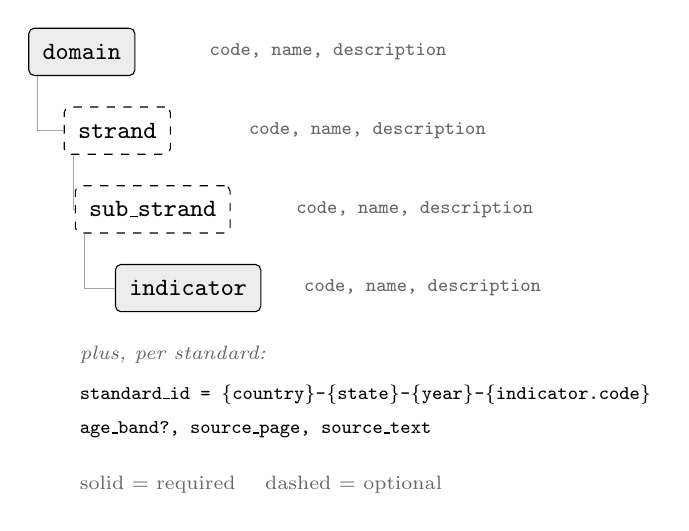
\begin{tikzpicture}[
  font=\small,
  lvl/.style={draw, rounded corners=2pt, minimum height=6mm, inner xsep=5pt, align=left},
  req/.style={lvl, fill=black!7},
  opt/.style={lvl, dashed, fill=white},
  ann/.style={font=\scriptsize\ttfamily, anchor=west, text=black!60},
  link/.style={-, gray!70}
]
\node[req] (d)  at (0,0)      {\texttt{domain}};
\node[opt] (s)  at (0.45,-1)  {\texttt{strand}};
\node[opt] (ss) at (0.90,-2)  {\texttt{sub\_strand}};
\node[req] (i)  at (1.35,-3)  {\texttt{indicator}};

\draw[link] (d.south west) ++(0.12,0) |- (s.west);
\draw[link] (s.south west) ++(0.12,0) |- (ss.west);
\draw[link] (ss.south west) ++(0.12,0) |- (i.west);

\node[ann] at (1.5,0)    {code, name, description};
\node[ann] at (2.0,-1)   {code, name, description};
\node[ann] at (2.6,-2)   {code, name, description};
\node[ann] at (2.7,-3)   {code, name, description};

\node[font=\scriptsize, anchor=west, text=black!60] at (-0.15,-3.85)
  {\textit{plus, per standard:}};
\node[font=\scriptsize\ttfamily, anchor=west] at (-0.15,-4.35)
  {standard\_id = \{country\}-\{state\}-\{year\}-\{indicator.code\}};
\node[font=\scriptsize\ttfamily, anchor=west] at (-0.15,-4.8)
  {age\_band?, source\_page, source\_text};

\node[font=\scriptsize, anchor=west, text=black!60] at (-0.15,-5.5)
  {solid = required \quad dashed = optional};
\end{tikzpicture}
\caption{The canonical schema. Four hierarchy levels, of which
\texttt{strand} and \texttt{sub\_strand} are optional; each carries a code, a
name and an optional description. A stored record is one indicator together
with its fully resolved ancestry, not a node in a tree (\S\ref{sec:schema}).}
\label{fig:schema}
\end{figure}


\section{Representative Golden Examples}
\label{sec:appendix-goldens}
% AUTO-GENERATED by paper/naacl2027/make_tables.py -- do not hand-edit.
% Every field is copied from the golden files on disk.

The detector golden is a flat list of elements and the parser golden a nested record per standard. The two examples below show the conventions \S\ref{sec:method-parsing} turns on; descriptions are omitted, and codes and identifiers are reproduced in full.
\medskip

{\raggedright\noindent\textbf{KY detector golden: a \texttt{<Label> <id>} heading, whose label-and-id is the code}\par}
\smallskip
{\scriptsize\noindent
\begin{tabular}{@{}p{0.22\linewidth}p{0.72\linewidth}@{}}
\toprule
\texttt{level} & \texttt{sub\_\allowbreak{}strand} \\
\texttt{code} & \texttt{Benchmark 1.\allowbreak{}1} \\
\texttt{title} & Maintains focus and sustains attention. \\
\bottomrule
\end{tabular}\par}
\medskip

{\raggedright\noindent\textbf{KY parser golden: the same element, its label form resolved to a domain-qualified code}\par}
\smallskip
{\scriptsize\noindent
\begin{tabular}{@{}p{0.3\linewidth}p{0.64\linewidth}@{}}
\toprule
\texttt{standard\_id} & \texttt{US-\allowbreak{}KY-\allowbreak{}2021-\allowbreak{}AL.\allowbreak{}1.\allowbreak{}1.\allowbreak{}EASPT} \\
\texttt{domain.code} & \texttt{AL} \\
\texttt{domain.name} & Approaches to Learning \\
\texttt{strand.code} & \texttt{AL.\allowbreak{}1} \\
\texttt{strand.name} & Sustains attention and persists with challenging activities and experiences. \\
\texttt{sub\_strand.code} & \texttt{AL.\allowbreak{}1.\allowbreak{}1} \\
\texttt{sub\_strand.name} & Maintains focus and sustains attention. \\
\texttt{indicator.code} & \texttt{AL.\allowbreak{}1.\allowbreak{}1.\allowbreak{}EASPT} \\
\texttt{indicator.name} & Engages in an activity for a sustained period of time. \\
\bottomrule
\end{tabular}\par}
\medskip

{\raggedright\noindent\textbf{NV parser golden: a printed namespace that skips a level, so the sub-strand code does not extend the strand's}\par}
\smallskip
{\scriptsize\noindent
\begin{tabular}{@{}p{0.3\linewidth}p{0.64\linewidth}@{}}
\toprule
\texttt{standard\_id} & \texttt{US-\allowbreak{}NV-\allowbreak{}2023-\allowbreak{}SS.\allowbreak{}ID.\allowbreak{}PK1} \\
\texttt{domain.code} & \texttt{SS} \\
\texttt{domain.name} & Social Studies \\
\texttt{strand.code} & \texttt{SS.\allowbreak{}1} \\
\texttt{strand.name} & Demonstrate a basic awareness of self as an individual, within the context of a group and community. \\
\texttt{sub\_strand.code} & \texttt{SS.\allowbreak{}ID} \\
\texttt{sub\_strand.name} & Individual Development and Cultural Identity \\
\texttt{indicator.code} & \texttt{SS.\allowbreak{}ID.\allowbreak{}PK1} \\
\texttt{indicator.name} & Identify and describe characteristics of self that are unique from others. \\
\bottomrule
\end{tabular}\par}
\medskip


\section{Confidence Score Distribution}
\label{sec:appendix-confidence}

Detection emits a confidence score, but nothing in the pipeline reads it.
Table~\ref{tab:confidence-distribution} gives its distribution by hierarchy
level and by audit verdict. Across 379 elements the score takes only five
distinct values, all in $[0.90, 0.97]$, and the band the prompt reserves for
guesses is never used. The lowest-confidence state, Kentucky, is perfect on
recall, code accuracy and precision. A threshold would therefore filter on
noise, so instead every record carries its source page and per-level
verification state, and all records are reviewed by a person. The score
also drifts between runs: on an earlier freeze of the same corpus, 89.7\% of
indicators scored 0.95 or above, against 93.5\% in the recorded run. The single
confirmed hallucination is the lowest-scoring element (0.90), but with one
invented element in the corpus no threshold's false-negative rate is
measurable.

% AUTO-GENERATED by paper/naacl2027/make_tables.py -- do not hand-edit.
% Source: paper/results/task8_20260904/confidence_distribution.json
% Regenerate with: python paper/naacl2027/make_tables.py
\begin{table}[t]
  \centering
  \small
  \begin{tabular}{lrrr}
    \toprule
    & $n$ & \textbf{Range} & $\mathbf{\geq 0.95}$ \\
    \midrule
    \multicolumn{4}{l}{\emph{By hierarchy level}} \\
    domain & 16 & 0.95--0.97 & 16/16 \\
    strand & 51 & 0.92--0.97 & 48/51 \\
    sub-strand & 49 & 0.92--0.97 & 47/49 \\
    indicator & 263 & 0.90--0.97 & 246/263 \\
    \midrule
    \multicolumn{4}{l}{\emph{By audit verdict (in-scope only)}} \\
    matched a golden & 135 & 0.92--0.97 & 117/135 \\
    real, unannotated & 117 & 0.92--0.97 & 115/117 \\
    real, split title & 39 & 0.95--0.96 & 39/39 \\
    real, reprinted & 5 & 0.95 & 5/5 \\
    \textbf{invented} & 1 & 0.90 & 0/1 \\
    \midrule
    All & 379 & 0.90--0.97 & 357/379 \\
    \bottomrule
  \end{tabular}
  \caption{Detector self-reported confidence over the 379 elements of the recorded run (subset tier). The verdict rows cover the 297 detections inside the domains a golden annotates; the other 82 were not audited. The prompt asks for $\geq 0.95$ when the depth map clearly applies, $0.80$--$0.94$ when the chunk is ambiguous, and $<0.70$ when guessing; the score takes 5 distinct values in $[0.90, 0.97]$ and uses the bottom band never. \textbf{Nothing in the pipeline thresholds this score} (\S\ref{sec:lessons}).}
  \label{tab:confidence-distribution}
\end{table}


\section{Corpus}
\label{sec:appendix-corpus}

Table~\ref{tab:corpus-appendix} identifies every source document, and
Table~\ref{tab:corpus-pages} the pages each tier retains, so either tier can be
reconstructed from the issuing agency's copy.

% AUTO-GENERATED by paper/naacl2027/make_tables.py (via generate_tables.build_corpus_appendix_table) -- do not hand-edit.
% Source: standards/standards_tracking.md, paper/results/corpus_tiers.json
% Regenerate with: python paper/analysis/generate_tables.py
% Corpus tier (guardrail 1): every row is the _only_subset tier, never full-document.
\begin{table*}[t]
\centering
\small
\begin{tabular}{llrlrrr}
\toprule
\textbf{State} & \textbf{Role} & \textbf{Year} & \textbf{Publisher} & \textbf{Full} & \textbf{Trim.} & \textbf{Subset} \\
\midrule
CA & dev & 2021 & CA Dept.\ of Education & 68 & -- & 13 \\
AZ & dev & 2018 & AZ Dept.\ of Education & 217 & 65 & 15 \\
TX & dev & 2022 & TX Education Agency & 87 & 71 & 9 \\
CO & dev & 2020 & CO Dept.\ of Early Childhood & 41 & 41 & 10 \\
NV & validation & 2023 & NV Dept.\ of Education & 98 & 71 & 15 \\
KY & validation & 2021 & Governor's Office of Early Childhood & 120 & 52 & 8 \\
\bottomrule
\end{tabular}
\caption{Corpus provenance. \emph{Full} is the published PDF; \emph{Trim.}\ removes non-standards matter while retaining every standard; \emph{Subset} is the one-to-two-domain excerpt the headline quality measurements use, and is a genuine reduction in coverage. Colorado's \emph{Full} is its 41-page Ages~3--5 publication (\S\ref{sec:corpus}). These are third-party state-agency documents, identified here rather than redistributed (\S\ref{sec:artifacts-statement}).}
\label{tab:corpus-appendix}
\end{table*}

% AUTO-GENERATED by paper/naacl2027/make_tables.py -- do not hand-edit.
% Source: paper/results/corpus_page_ranges.json
% Regenerate with: python paper/naacl2027/make_tables.py
\begin{table*}[t]
\centering
\small
\begin{tabular}{llrp{0.62\textwidth}}
\toprule
\textbf{State} & \textbf{Tier} & \textbf{pp} & \textbf{Retained PDF pages} \\
\midrule
AZ & trimmed & 65 & 2, 21, 23--28, 41, 43--50, 66, 70--82, 107, 110--120, 139, 142--145, 156, 158--162, 179, 181--185, 198, 201--204 (of 217) \\
AZ & subset & 15 & 2, 21, 23, 66, 70--78, 81--82 (of 217) \\
CA & subset & 13 & 1--5, 11--13, 18--22 (of 68) \\
CO & trimmed & 41 & 1--41 (of 41) \\
CO & subset & 10 & 1, 3--9, 11--12 (of 41) \\
TX & trimmed & 71 & 1, 9--65, 69--81 (of 87) \\
TX & subset & 9 & 1, 9--13, 59--61 (of 87) \\
NV & trimmed & 71 & 1, 3, 16--84 (of 98) \\
NV & subset & 15 & 1, 3, 23--26, 54--57, 61--65 (of 98) \\
KY & trimmed & 52 & 1, 52--102 (of 120) \\
KY & subset & 8 & 1, 52--55, 65, 71--72 (of 120) \\
\bottomrule
\end{tabular}
\caption{Pages each tier retains, as indices into the published PDF file. Printed page numbers differ by each document's front matter (Kentucky's PDF page 52 is printed page 39). Every tier page was matched by text to a published page. California has no trimmed tier.}
\label{tab:corpus-pages}
\end{table*}


\section{Deployed Architecture}
\label{sec:appendix-architecture}

% Deployed architecture, full width, read left to right. Hand-authored TikZ:
% it depicts the deployed topology, not measured data. Replaces the review
% build's use of ../figures/fig_architecture.pdf
% (paper/analysis/make_architecture_figure.py), whose labels shrank to 1.9pt at
% text width. Keep in sync with documentation/ARCHITECTURE.md: ten Lambda
% handlers (the gray boxes), Pass 1 runs in the detection prepare handler, and
% every stage boundary is an S3 write and read.
%
% Geometry is explicit so the six cards fit \textwidth (16cm) at 8pt text:
% four single-handler cards 1.95cm wide, two batched cards 2.8cm, 0.38cm gaps.
\begin{figure*}[t]
\centering
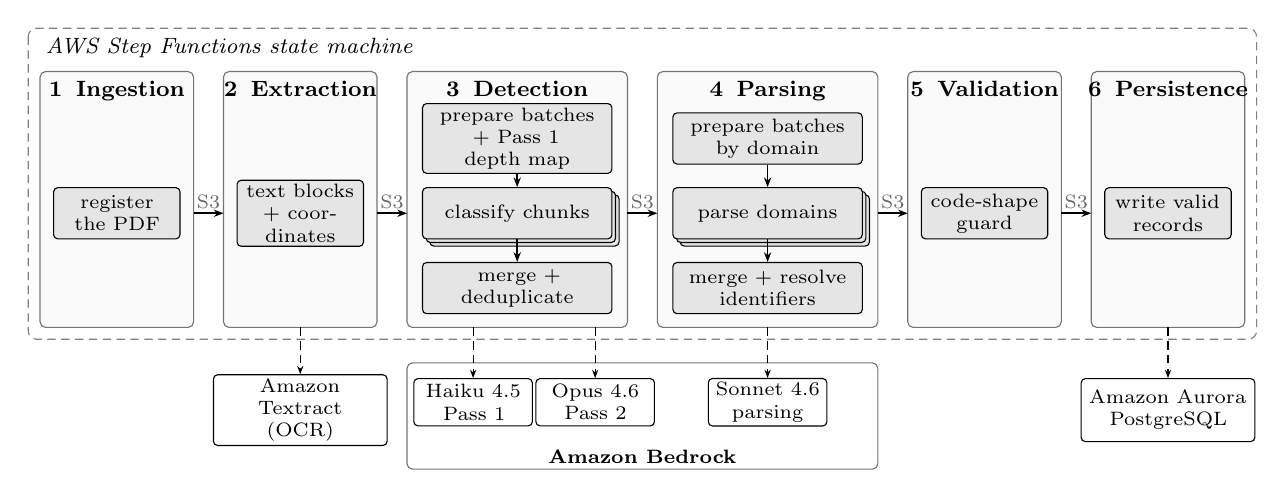
\begin{tikzpicture}[
  x=1cm, y=1cm,
  card/.style={draw=black!55, rounded corners=2pt, fill=black!2},
  ctitle/.style={font=\footnotesize\bfseries, anchor=north, inner sep=0pt},
  fn/.style={draw, rounded corners=1.5pt, fill=black!10, font=\scriptsize,
    align=center, text width=#1, minimum height=6.5mm, inner sep=1.5pt},
  fn/.default=15mm,
  mapfn/.style={fn=#1, double copy shadow={shadow xshift=1.3pt,
    shadow yshift=-1.3pt, fill=black!10, draw}},
  mapfn/.default=15mm,
  svc/.style={draw, rounded corners=1.5pt, fill=white, font=\scriptsize,
    align=center, text width=#1, minimum height=8mm, inner sep=1.5pt},
  svc/.default=17mm,
  flow/.style={-{Stealth[length=3.5pt]}, semithick},
  call/.style={-{Stealth[length=3pt]}, densely dashed},
  s3/.style={font=\scriptsize, text=black!60, above, inner sep=1.5pt},
]
% Card spans (left, right) and centers.
\def\cardA{0}     \def\cardAr{1.95}   \def\cA{0.975}
\def\cardB{2.33}  \def\cardBr{4.28}   \def\cB{3.305}
\def\cardC{4.66}  \def\cardCr{7.46}   \def\cC{6.06}
\def\cardD{7.84}  \def\cardDr{10.64}  \def\cD{9.24}
\def\cardE{11.02} \def\cardEr{12.97}  \def\cE{11.995}
\def\cardF{13.35} \def\cardFr{15.30}  \def\cF{14.325}
\def\ctop{0}      \def\cbot{-3.25}    \def\cmid{-1.8}

% Orchestration frame.
\draw[black!50, densely dashed, rounded corners=3pt]
  (-0.15, 0.55) rectangle (15.45, -3.4);
\node[font=\footnotesize\itshape, anchor=west] at (-0.05, 0.3)
  {AWS Step Functions state machine};

% Stage cards.
\foreach \l/\r/\c/\t in {\cardA/\cardAr/\cA/1\enspace Ingestion,
                         \cardB/\cardBr/\cB/2\enspace Extraction,
                         \cardC/\cardCr/\cC/3\enspace Detection,
                         \cardD/\cardDr/\cD/4\enspace Parsing,
                         \cardE/\cardEr/\cE/5\enspace Validation,
                         \cardF/\cardFr/\cF/6\enspace Persistence} {
  \draw[card] (\l, \ctop) rectangle (\r, \cbot);
  \node[ctitle] at (\c, \ctop - 0.12) {\t};
}

% Lambda handlers: one per single-handler card, three per batched card.
\node[fn] (ing) at (\cA, \cmid) {register\\ the PDF};
\node[fn] (ext) at (\cB, \cmid) {text blocks\\ + coordinates};
\node[fn=23mm] (dprep) at (\cC, -0.85) {prepare batches\\ + Pass 1 depth map};
\node[mapfn=23mm] (dmap) at (\cC, \cmid) {classify chunks};
\node[fn=23mm] (dmerge) at (\cC, -2.75) {merge + deduplicate};
\node[fn=23mm] (pprep) at (\cD, -0.85) {prepare batches\\ by domain};
\node[mapfn=23mm] (pmap) at (\cD, \cmid) {parse domains};
\node[fn=23mm] (pmerge) at (\cD, -2.75) {merge + resolve\\ identifiers};
\node[fn] (val) at (\cE, \cmid) {code-shape\\ guard};
\node[fn] (per) at (\cF, \cmid) {write valid\\ records};

\draw[flow] (dprep) -- (dmap);
\draw[flow] (dmap) -- (dmerge);
\draw[flow] (pprep) -- (pmap);
\draw[flow] (pmap) -- (pmerge);

% Stage to stage: every hand-off is a JSON write and read through S3.
\foreach \a/\b in {\cardAr/\cardB, \cardBr/\cardC, \cardCr/\cardD,
                   \cardDr/\cardE, \cardEr/\cardF} {
  \draw[flow] (\a, \cmid) -- node[s3] {S3} (\b, \cmid);
}

% External services. The Bedrock label sits at the bottom of its box so the
% call arrows from above never cross it.
\node[svc=21mm] (ocr) at (\cB, -4.3) {Amazon Textract\\ (OCR)};
\draw[black!55, rounded corners=2pt] (\cardC, -3.7) rectangle (\cardDr, -5.05);
\node[font=\scriptsize\bfseries, anchor=south, inner sep=2pt]
  at ({(\cardC+\cardDr)/2}, -5.05) {Amazon Bedrock};
\node[svc=14mm, minimum height=6mm] (haiku) at (5.5, -4.2) {Haiku 4.5\\ Pass 1};
\node[svc=14mm, minimum height=6mm] (opus) at (7.05, -4.2) {Opus 4.6\\ Pass 2};
\node[svc=14mm, minimum height=6mm] (sonnet) at (\cD, -4.2) {Sonnet 4.6\\ parsing};
\node[svc=21mm] (db) at (\cF, -4.3) {Amazon Aurora\\ PostgreSQL};

\draw[call] (\cB, \cbot) -- (ocr);
\draw[call] (5.5, \cbot) -- (haiku);
\draw[call] (7.05, \cbot) -- (opus);
\draw[call] (\cD, \cbot) -- (sonnet);
\draw[call] (\cF, \cbot) -- (db);
\end{tikzpicture}
\caption{Deployed architecture, read left to right. Each gray box is one of the
ten AWS Lambda handlers; stacked boxes fan out through a Step Functions
\texttt{Map} state with at most three concurrent workers. Every hand-off between
stages is a JSON write and read through Amazon S3. Dashed arrows are calls to
external services; only records that pass validation are persisted.}
\label{fig:architecture}
\end{figure*}


Figure~\ref{fig:architecture} shows the deployed system: ten Lambda handlers
orchestrated by Step Functions, with every stage boundary an S3 write and read,
Bedrock model calls in detection and parsing, and Aurora PostgreSQL Serverless
as the store. Only records that pass validation reach persistence.

All model calls go through Amazon Bedrock at temperature zero, using these
model identifiers:

{\small
  \begin{itemize}
      \setlength{\itemsep}{0pt}
    \item depth map:\\ \texttt{us.anthropic.claude-haiku-4-5-20251001-v1:0}
    \item detection:\\ \texttt{us.anthropic.claude-opus-4-6-v1}
    \item parsing:\\ \texttt{us.anthropic.claude-sonnet-4-6}
\end{itemize}}

\end{document}
